\documentclass[11pt]{report}

\usepackage{graphicx}
\usepackage[utf8]{inputenc}


\begin{document}
\title{Virtual Reality}
\author{Maximilian Sieß}
\maketitle

\tableofcontents

%\chapter{Abstract}

\chapter{Introduction}
Virtual Reality is the attempt to use technology, such as head mounted display devices, and computer generated graphics, to allow the user to experience a sense of presence in a virtual environment. This is used in a wide variety of cases, including but not limited to, entertainment, education, medical therapy, research, and visualization.

\chapter{Related Work}
\section{Headmounted Display Technology}
	The concept of Virtual Reality dates back to the 1980s (Citation Needed), and unlike some depiction of it in pop culture at the time, never archived the level of immersion and presence that recent technological advances enable us to. Due to a jump in interest hardware such as the Oculus Rift found funding in recent years. In the case of Oculus, it was via Crowdfunding. But as a result, commercial products from Google, Valve/HTC or Sony have been announced. At the time of writing, none of the mentioned companies have released a commercially available end user product. Oculus Rift has released and sold Developer Kits, which are most frequently used in modern Virtual Reality endeavours.

	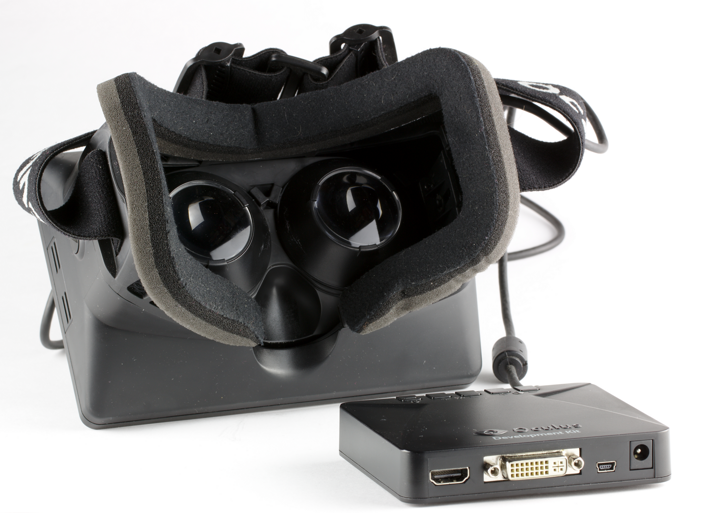
\includegraphics[scale=0.3]{or_small}

\section{Software}
	Programming software for virtual reality does not differ much from regular computer graphics programming. Most commercial vendors offer their own API that helps translating a virtual camera to a two camera 3D setup. It was found however, that how the camera is used is imperitive to not give the user of the virtual reality headsead motion sickness. For example, moving the camera without the user moving their head was resulted in severly negative feedback from the test subjects.
	
\section{Additional Hardware}
With headmounted displays, vision, the groundwork for a feeling of presence in virtual reality, is laid out. Headsets or surround sound systems have been shown to suffice for the audio representation of the virtual environment.\\
Moving around naturally has proven difficult, however. While video game demos often use a gamepad, it is less than ideal for upholding a sense of presence. Products, such as the XYZ try to enable free movement in virtual reality.



	%\section{Entertainment}
	%Oculus rift, Valve, Project Morpheus - VIDJA GAMES!
	
	%\section{Education}
	%Look at papers you downloaded
	
	%\section{Therapy}
	%Look at papers or download more!
	
	%\section{Research}
	%Papers!
	
	%\section{Visualization}
	%You know, like for surgery, architecture and stuffs.


\chapter{Discussion}
%How helpful is it now? Will it be real reality soon? how soon? absolute presence is not possible with just a headmount set, so wtf Valve, where is my absolute-immersion-set that lets me LittlePip and shoot down some raiders, eh?

	\begin{equation}
		x - x_i = \sqrt{\frac{k^2}{2}} \int_0^1 \frac{1}{\sqrt{1-\sin^2 \phi}} d\phi
	\end{equation}

%\chapter{Conclusion}

\chapter{References}

%\chapter{Appendix}

%\bibliographystyle{plain}
\begin{bibliography}{9}

	\bibitem{zyda05}
  	Micheal Zyda:
  	\emph{From Visual Simulation to Virtual Reality},
  	Published in Computer Volume 38, Issue 9,
  	September 2005
  	
  	\bibitem{bailey14}
  	Lisa Avila, Mike Bailey:
  	\emph{Virtual Reality for the Masses},
  	Published in IEEE Computer Graphics and Applications,
  	September 2014
  	
  	\bibitem{ruddle13}
  	Roy A. Ruddle, Ekaterina Volkova, Heinrich H. Bülthoff:
  	\emph{Learning to Walk in Virtual Reality},
  	ACM Transactions on Applied Percecption, Vol 10, No. 2, Article 11
  	May 2013
  	
  	\bibitem{leck13}
  	Kathy Leck:
  	\emph{Giving Students Real-World Experience via Virtual-Reality Learning },
  	Published in eLearn Magazine,
  	May 2013, \\
  	\hyperlink{http://elearnmag.acm.org/archive.cfm?aid=2484903}
  	
  	\bibitem{satava02}
  	Neal E. Seymour, MD,* Anthony G. Gallagher, PhD,† Sanziana A. Roman, MD,* Michael K. O’Brien, MD,* Vipin K. Bansal, MD,*
Dana K. Andersen, MD,* and Richard M. Satava, MD*:
  	\emph{Virtual Reality Training Improves Operating Room Performance},
  	Published in Annals of Surgery,
  	Volume 236, No. 4,
  	2002

	\bibitem{beltran13}
  	Marta Beltrán:
  	\emph{The Importance of the Avatar Gender in Training Simulators Based on Virtual Reality},
  	Published in ITiCSE,
  	July 2013
  	

\end{bibliography}	
	

\end{document}
